\section{Fundamentals} 

\begin{frame}
	\frametitle{Search-based software testing}
	
	\begin{itemize}
		\item tests for object oriented languages
		\item sequence of method calls
		\item
		\item
		\item
	\end{itemize}
			
	
\end{frame}

\begin{frame}
	\frametitle{Fitness}
	
	\begin{columns}[c]
		
		\column{.45\textwidth}
		\blockheading{Fitness function}
				
		\begin{itemize}
			\item 
			\item function for e.g. coverage
			\item guidance for search algorithms
			\item
			\item
		\end{itemize}
		
		\column{.45\textwidth}
		\lstinputlisting{code/simple_guidance.java}

	\end{columns}
	
\end{frame}

\begin{frame}
	\frametitle{Fitness}
	
	\begin{columns}[c]
		
		\column{.45\textwidth}
		\blockheading{Fitness landscape}
				
		\begin{itemize}
			\item 
			\item 
			\item
			\item
			\item
		\end{itemize}
		
		\column{.45\textwidth}
		\begin{figure}
			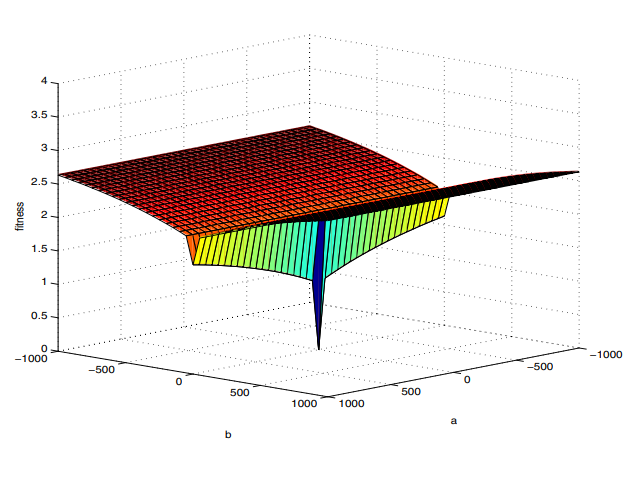
\includegraphics[width=1\textwidth]{figures/complex_landscape}
		\end{figure}
		
		
	\end{columns}
	
\end{frame}

\begin{frame}
	\frametitle{Genetic algorithm}
	
	\begin{columns}[c]
		
		\column{.45\textwidth}
		\blockheading{Heading}
		
		\begin{itemize}
			\item Statement
			\item Explanation
			\item Example
		\end{itemize}
		
		\column{.45\textwidth}
		\blockheading{Heading}
		
		\begin{itemize}
			\item Statement
			\item Explanation
			\item Example
		\end{itemize}	
		
	\end{columns}
	
\end{frame}

\begin{frame}
	\frametitle{DynaMOSA}
	
	\begin{columns}[c]
		
		\column{.45\textwidth}
		\blockheading{Heading}
		
		\begin{itemize}
			\item Statement
			\item Explanation
			\item Example
		\end{itemize}
		
		\column{.45\textwidth}
		\blockheading{Heading}
		
		\begin{itemize}
			\item Statement
			\item Explanation
			\item Example
		\end{itemize}	
		
	\end{columns}
	
\end{frame}